\subsection{Biologic neuron}

The human brain is a complex system that coordinates the behavior of the body. He could not be matched by any digital structure.

The functional unit of the creature is the neuron. In the human brain there are about $ 10 ^ {11} $ neurons. They transmit and receive electro-chemical signals.

A neuron is composed of: \cite{toulouse}:
\begin{itemize}
    \item A cell body (soma).
    \item Dendrite, which fulfills the input function, capture information.
    \item Axon, an extension of the neuron body, with output function.
\end{itemize}

The dendritic tree collects the input signals from other neurons; soma converts the input signals into output signals, and the axon transmits the output signals to other neurons. Neurons are interconnected with synapses.

Neurons communicate with each other through electrical signals. These are propagated along the axon until they encounter the synaptic bond. Dendrites of the biological neuron receive electrical signals from the axons of other neurons.

Neurotransmitter molecules reach the post-synaptic neuron membrane, where the intake of these molecules induce post-synaptic action potential (PSP) \cite{calculNeuronal}.

PSPs generated at various points of the dendritic tree diffuse through attenuation to the soma, where they are integrated. If the total amount of PSPs embedded within a short time span exceeds a certain threshold of about a few tens of minivolts, called activation level, the neuron will become active, generating a potential for action along the axon.

The contribution of an input signal to PSP characterizes the size called synaptic strength or synaptic efficiency. Such an input signal has a value of about 1 minivolt, which may be an excitatory signal or an inhibitory signal, depending on the positive or negative influence it has on making a neuron to become active. We must point out that the PSP is not unique determined by the input signal. Different noise sources, in relation to the chemical neurotransmitter quantity fluctuations released on the synaptic connection, involve a probabilistic input-output relationship.

The time interval between the moment of a signal transmission to the pre-synaptic neuron soma and the time of emission of a signal induced by the postsynaptic neuron is approximately 1-2 ms. It follows that a neuron can have a maximum emission of about 500-1000 signals per second, which is reduced by about 3-5 times in a neural network.

From these dynamics considerations of neuronal activity, one can notice that biological neuron is a slow biological device compared to man-made electronic devices - they can be even hundreds of thousands of times faster than a biological neuron. However, any computer-based computing system has lower brain performance than neurons. The obvious conclusion is that the computing power of the human brain is not due to the processing speed of constitutive neurons but to the wide interconnection of slow biological devices - neurons, which perform simple operations: integration of incoming signals along the dendritic tree and emission of a signal along the axon, if the integrated input signal exceeds the activation level \cite{calculNeuronal}.

\begin{figure}[H]
  \centering
  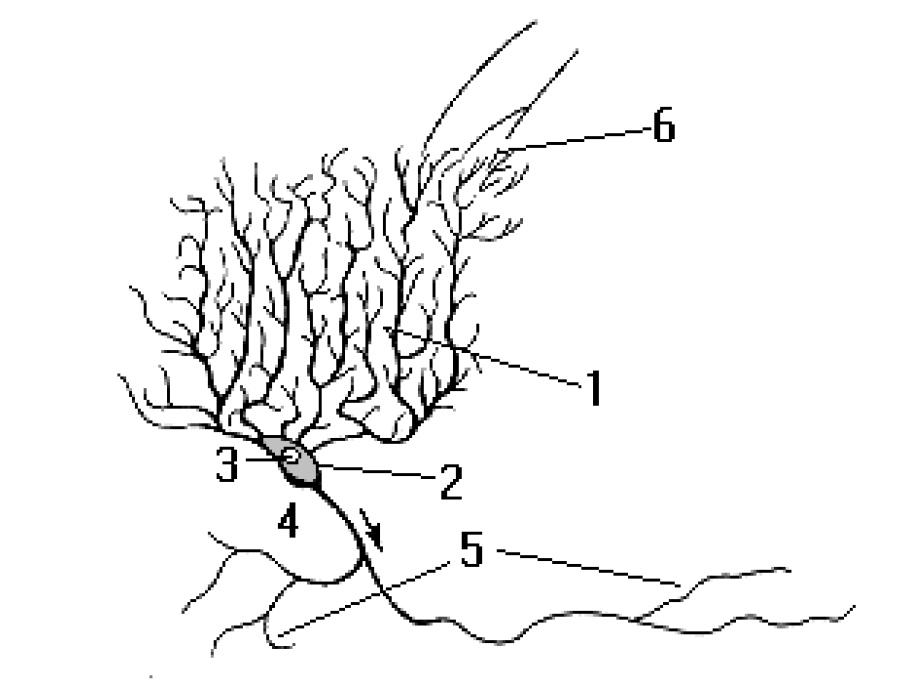
\includegraphics[width=3.5in]{images/neuronulBiologic.png}
  \caption {
      Schematic representation of the biological neuron.\\ 
      1 - The dendritic tree;\\ 
      2 - Soma (cell body);\\ 
      3 - The core of the neuronal cell;\\ 
      4 - The axon;\\ 
      5 - The axon tree;\\ 
      6 - Synaptic connections.
  }
\end{figure}

Changing synaptic strength is the result of a "learning" process \cite{calculNeuronal}. Link synaptic and signal processing by the neuron form the mechanism of based on the memory capacity of the brain.